\section{Feature Extraction} \label{sec:featureextract}
The binary blob mask of an object contains too much redundant information for the tracking algorithm. As reviewed in \autoref{ch:review}, a binary blob could be represented as a feature vector of the centroid and the size, denoted as \autoref{eq:blobdenote1}, where $C$ is the 2D coordinate of the geometry center and $S$ is the total pixel number of the blob.
\begin{equation}\label{eq:blobdenote1}
  B = \{C,S\}
\end{equation}

This basic representation is sufficient for a single object tracking because the centroid is a unique feature for a blob. However, when two objects overlap and their blob masks merge together, they will be regarded as one single blob and therefore have only one shared centroid. The uniqueness of the centroid no longer holds, and the one-to-one matching relation between an object and its corresponding blob mask is broken.
\autoref{fig:blobmerge} shows an example demonstrating how the merged blobs impede the feature extraction. In the first two frames where two blobs are not merged, their centroids remain unique and transit a small shift from the last frame. The size of the blobs remain similar as the last frame as well. In the third frame, the blobs are merged, their centroids disappear and is replaced with a single centroid at the center of two blobs. Viewing the extracted feature only, we may only conclude that there is one blob with twice the size as before. Furthermore, the location of the centroid jumps abruptly, not close to either centroids in the last frame. In the fifth frame, the blobs are again separated. An abrupt change in centroid position takes place again.

Since the tracker match objects with its nearest neighbour in the last frame, a distance that is too long will break the matching. Even if the blobs are successfully matched, a shared centroid will bring ambiguity to the label assignment. Labels may be exchanged between two objects after splitting.
\begin{figure}
  \centering
  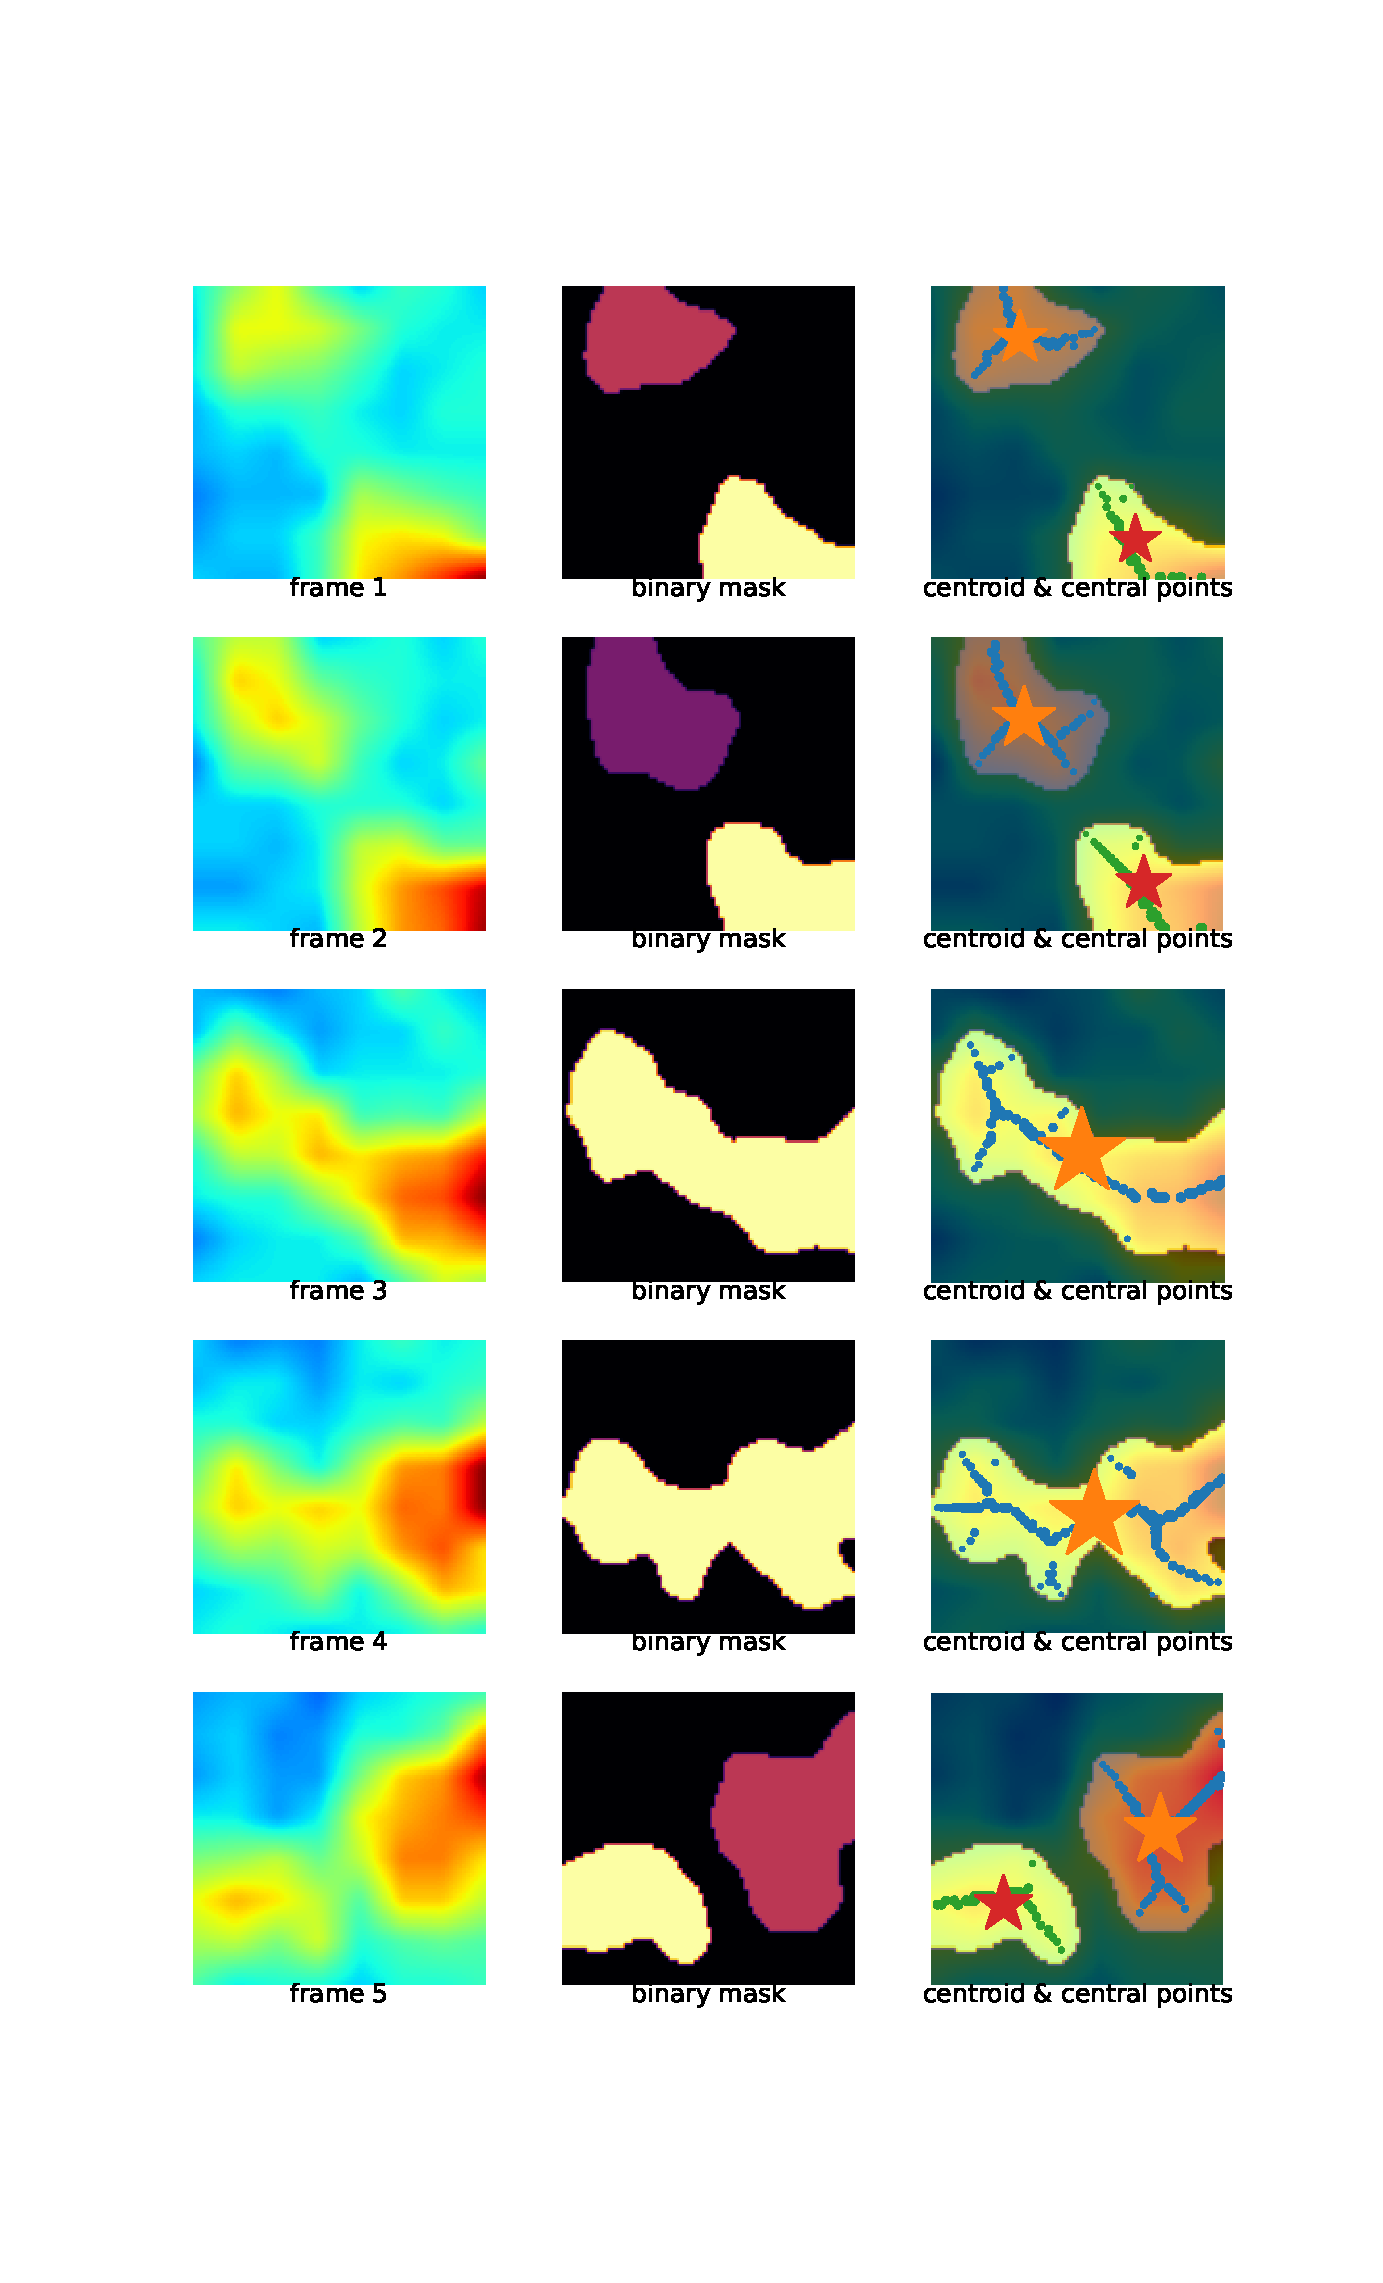
\includegraphics[width=0.6\textwidth]{figures/blobmerge.eps}
  \caption{An example frame sequence showing the blob merging issue. Left column is the interpolated image, middle column is the blob masks and right column shows the extracted feature. The star symbol represents the centroid location and the size of the start represents the size of the blob. Other round dots scattered inside the blob represent central points.}\label{fig:blobmerge}
\end{figure}

We follow the research of \cite{sharma2012blob}, adding ``central points'' as addition feature for blob representation. Central points of a blob are those points that are far away from the background, they can be found out by picking local maxima in a distance transform of the blob mask.
\subsection{introduction of distance transform}
A distance transform of a binary image labels every pixel of the image by the distance between that pixel and the nearest background pixel \cite{bailey2004efficient}, which could be denoted as \autoref{eq:distancetransform}.
\begin{equation}\label{eq:distancetransform}
  I_d(x,y) = \left\{\begin{array}{cc}
               0 & I(x,y)\in\{Bg\} \\
               \min\left(\Vert x-x_0,y-y_0\Vert\right),\forall I(x_0,y_0)\in Bg & I(x,y)\in\{Ob\}
             \end{array}\right.
\end{equation}
The $\Vert\cdot\Vert$ symbol is a distance definition, could be $L_1$, $L_2$, $L_{max}$ or any other distance metric. To our concern, the distance is measured in Euclidean metric, namely $\Vert x,y\Vert=\sqrt{x^2+y_2}$.

A precise computation of the Euclidean distance transform is complex. A commonly used approximation is the chamfer distance transform \cite{butt1998optimum}. The chamfer distance transform exploits the fact that the distance between of each pixel to its nearest background pixel depends on the previously computed neighbour. The whole distance transform image could be obtained in two pass, one propagating from the upper-left corner to the lower-right corner and the other reversely.

\begin{table}
  \centering
  \begin{tabular}{|c|c|c|}
    \hline
    % after \\: \hline or \cline{col1-col2} \cline{col3-col4} ...
    b & a & b \\
    a & $x_-$ & - \\
    - & - & - \\
    \hline
  \end{tabular}
  \begin{tabular}{|c|c|c|}
  \hline
    % after \\: \hline or \cline{col1-col2} \cline{col3-col4} ...
    - & - & - \\
    - & $x_+$ & a \\
    b & a & b \\
    \hline
  \end{tabular}
  \caption{Distance increment of two pass respectively for a $3\times3$ window.}\label{tab:chamfertable}
\end{table}

\subsection{local maxima in a distance transform}

\subsection{central points - an informative and stable representation}
Central points preserve most information about the original blob. If the distance value to the background of every central point is preserved, the original blob mask could be approximately recovered from the central points, see \autoref{fig:maskrecover}. In contrary, the shape information is lost when using the centroid representation. Certainly, multiple central points requires more memory space than a single centroid, but the central points representation compresses information efficiently.
 
The cluster of central points looks like the ``spine'' of the original blob.
\begin{figure}
  \centering
  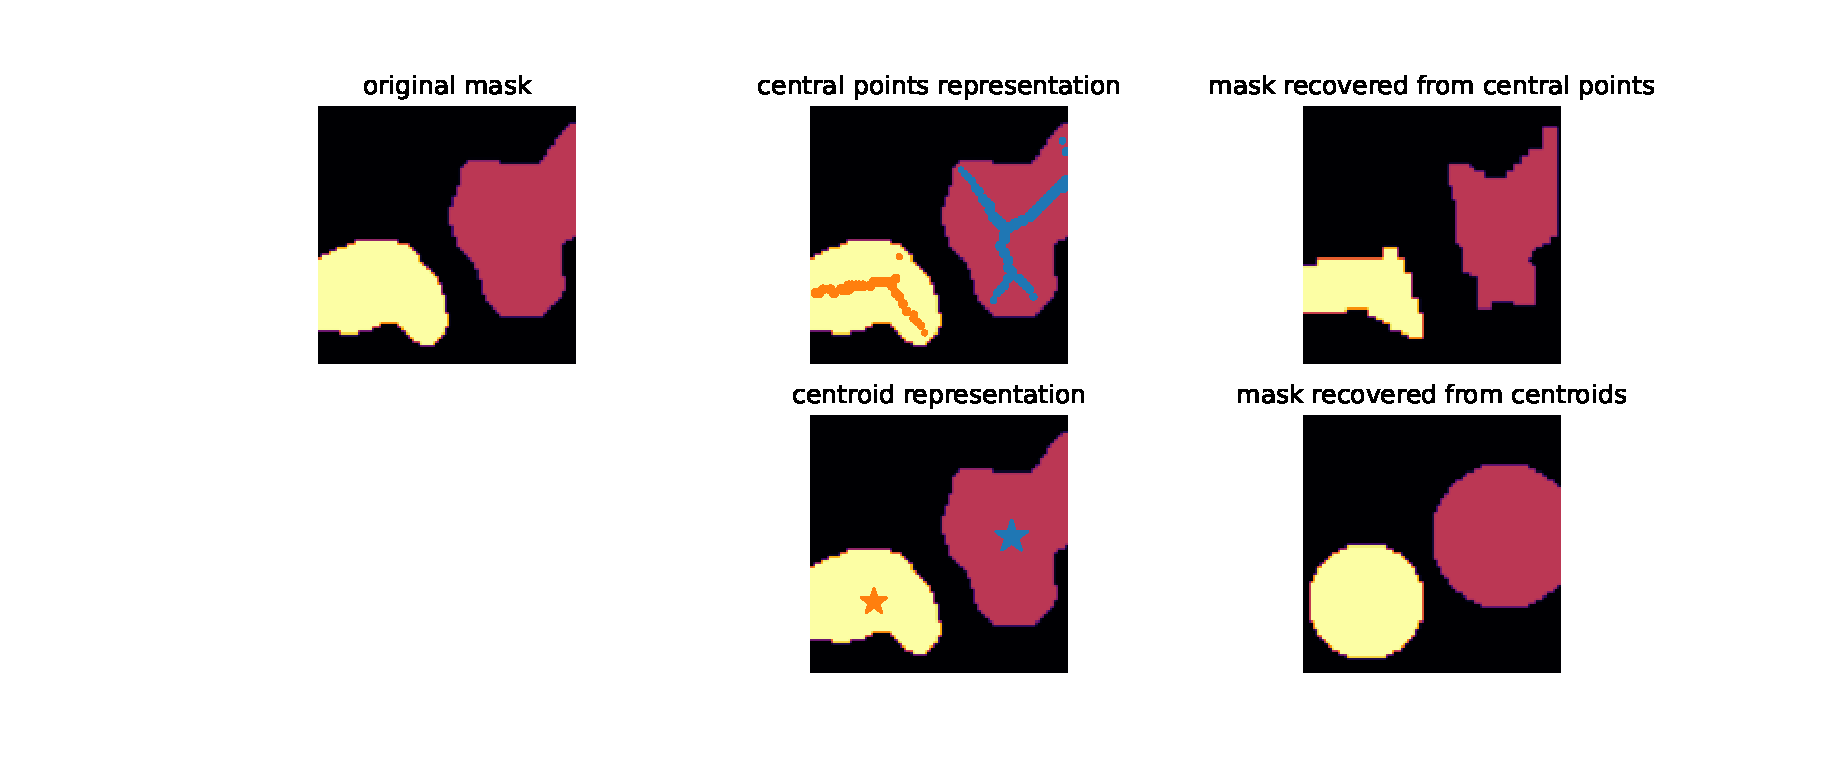
\includegraphics[width=\textwidth]{figures/maskrecover.eps}
  \caption{mask recover}\label{fig:maskrecover}
\end{figure}

